% This version of CVPR template is provided by Ming-Ming Cheng.
% Please leave an issue if you found a bug:
% https://github.com/MCG-NKU/CVPR_Template.

% \documentclass[review]{cvpr}
\documentclass[final]{cvpr}

\usepackage{times}
\usepackage{epsfig}
\usepackage{graphicx}
\usepackage{amsmath}
\usepackage{amssymb}
\usepackage{booktabs}
\usepackage{multirow}

% Include other packages here, before hyperref.

% If you comment hyperref and then uncomment it, you should delete
% egpaper.aux before re-running latex.  (Or just hit 'q' on the first latex
% run, let it finish, and you should be clear).
\usepackage[pagebackref=true,breaklinks=true,colorlinks,bookmarks=false]{hyperref}

%\setcounter{page}{4321} % For final version only


\begin{document}

%%%%%%%%% TITLE
\title{Image Processing and Computer Vision (CSC6051/MDS5112)  \\ Assignment 2}

\author{Qiheng Peng\\
Student ID: 225040065\\
{\tt\small 225040065@link.cuhk.edu.cn}
}

\maketitle


%%%%%%%%% ABSTRACT
\begin{abstract}
This report presents the implementations and experiments for Assignment 2, including Gaussian filtering (Task 1), global/local histogram equalization (Task 2), and monocular depth estimation on ScanNet (Task 3). For Task 1 and Task 2, I implemented all required operations in NumPy without using prohibited high-level APIs and visualized the qualitative effects. For Task 3, I trained a ResNet50-based baseline and evaluated it with aligned AbsRel, then performed a data-scale study under four training schedules, and finally compared with two foundation models (VGGT and Depth Anything 3). The results show that increasing training data while reducing epochs improved the baseline performance on the validation split in this setup, and foundation-model performance varied significantly depending on model/task alignment.
\end{abstract}

%-------------------------------------------------------------------------
\section{Task 1}

\paragraph{Implementation Details}
I implemented Gaussian filtering from scratch in \texttt{task1/task1.py}. The key steps are:
\begin{itemize}
   \item Input validation: checks for null input, odd kernel size greater than 1, and non-negative $\sigma$.
   \item Kernel generation: builds a 2D Gaussian kernel with
   \begin{equation}
      G(x,y)=\exp\left(-\frac{x^2+y^2}{2\sigma^2}\right),
   \end{equation}
   then normalizes it so that the kernel sums to 1.
   \item Convolution: applies sliding-window weighted sum with \texttt{reflect} padding.
   \item Data type restoration: clips the output to $[0,255]$ and converts back to original image type.
\end{itemize}
Both grayscale and RGB images are supported (channel-wise convolution for RGB).


\paragraph{Results \& Analysis}
I tested with \texttt{kernel\_size=5} and \texttt{sigma=1}. The output image is smoother and high-frequency noise/textures are reduced while keeping major structures intact.

\begin{figure}[htbp]
   \centering
   \begin{minipage}{0.48\linewidth}
      \centering
      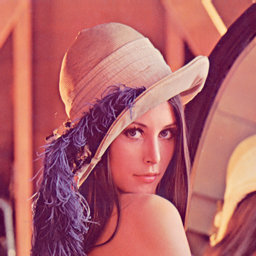
\includegraphics[width=\linewidth]{../task1/Lena-RGB.jpg}
      \caption*{(a) Input}
   \end{minipage}
   \hfill
   \begin{minipage}{0.48\linewidth}
      \centering
      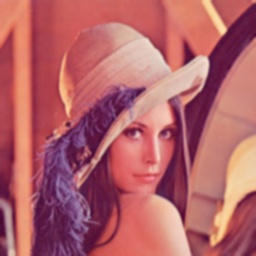
\includegraphics[width=\linewidth]{../task1/gaussian_result.jpg}
      \caption*{(b) Gaussian result}
   \end{minipage}
   \caption{Task 1 qualitative result of Gaussian filtering.}
   \label{fig:task1_result}
\end{figure}


%-------------------------------------------------------------------------
\section{Task 2}

\paragraph{Implementation Details}
I implemented both global and local histogram equalization in \texttt{task2/task2.py}.

\textbf{Global histogram equalization.}
\begin{itemize}
   \item Compute histogram $h(i)$ for $i\in[0,255]$.
   \item Compute CDF $c(i)=\sum_{j=0}^{i}h(j)$.
   \item Build LUT using
   \begin{equation}
      \hat{i}=\mathrm{round}\left(\frac{c(i)-c_{\min}}{N-c_{\min}}\cdot255\right),
   \end{equation}
   where $N$ is the number of pixels and $c_{\min}$ is the first non-zero CDF value.
\end{itemize}

\textbf{Local histogram equalization.}
\begin{itemize}
   \item Use a square window ($31\times31$) centered at each pixel.
   \item Compute local histogram/CDF and map current pixel by local CDF.
   \item Use reflect padding for border handling.
   \item Use a sliding-window histogram update (subtract left column and add right column) to reduce repeated computation.
\end{itemize}


\paragraph{Results \& Analysis}
Compared with global equalization, local equalization enhances local contrast more aggressively and reveals weak details in dark/flat regions. However, it may also amplify local noise and texture, which is consistent with adaptive histogram equalization behavior~\cite{wiki_hist_eq,wiki_adaptive_hist_eq}.

\begin{figure}[htbp]
   \centering
   \begin{minipage}{0.32\linewidth}
      \centering
      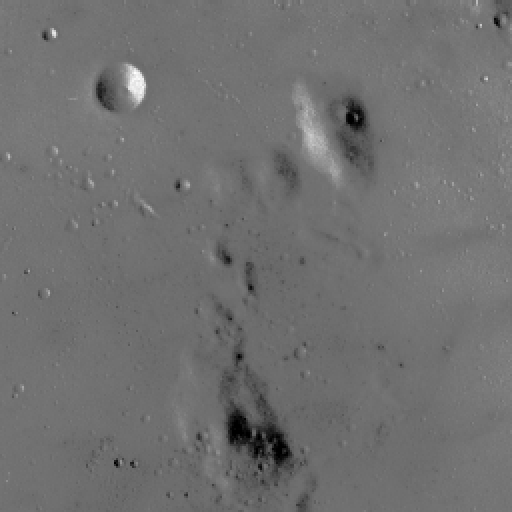
\includegraphics[width=\linewidth]{../task2/moon.png}
      \caption*{(a) Input}
   \end{minipage}
   \hfill
   \begin{minipage}{0.32\linewidth}
      \centering
      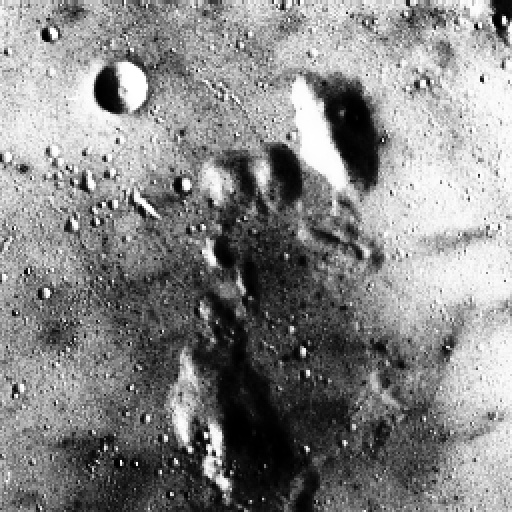
\includegraphics[width=\linewidth]{../task2/HistEqualization.jpg}
      \caption*{(b) Global HE}
   \end{minipage}
   \hfill
   \begin{minipage}{0.32\linewidth}
      \centering
      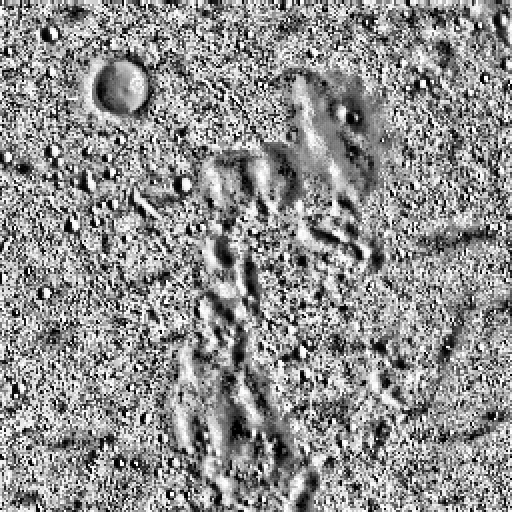
\includegraphics[width=\linewidth]{../task2/LocalHistEqualization.jpg}
      \caption*{(c) Local HE}
   \end{minipage}
   \caption{Task 2 comparison: local histogram equalization improves local details more strongly than global equalization.}
   \label{fig:task2_result}
\end{figure}


%-------------------------------------------------------------------------
\section{Task 3}

\paragraph{Setup and Protocol}
The training/evaluation pipeline is implemented in \texttt{task3/train.py} and \texttt{task3/test.py}. Following the assignment requirement, I trained the baseline model on ScanNet with the provided split files and reported aligned AbsRel~\cite{pytorch_basics,pytorch_docs}. The default baseline uses a ResNet50 encoder-decoder depth network with SiLog loss.

For evaluation, predictions are first aligned to ground-truth depth using per-image scale-shift least squares, then AbsRel is computed on valid pixels. All quantitative results below come from the JSON logs in \texttt{task3/outputs/*}.

\paragraph{Baseline and Data-Scale Study}
The baseline setting is 32 epochs with 10k max training samples. I additionally trained four settings required by the assignment:
\begin{itemize}
   \item 16 epochs + 20k samples,
   \item 8 epochs + 40k samples,
   \item 4 epochs + 80k samples,
   \item 2 epochs + 160k samples.
\end{itemize}

\begin{figure}[htbp]
   \centering
   \begin{minipage}{0.49\linewidth}
      \centering
      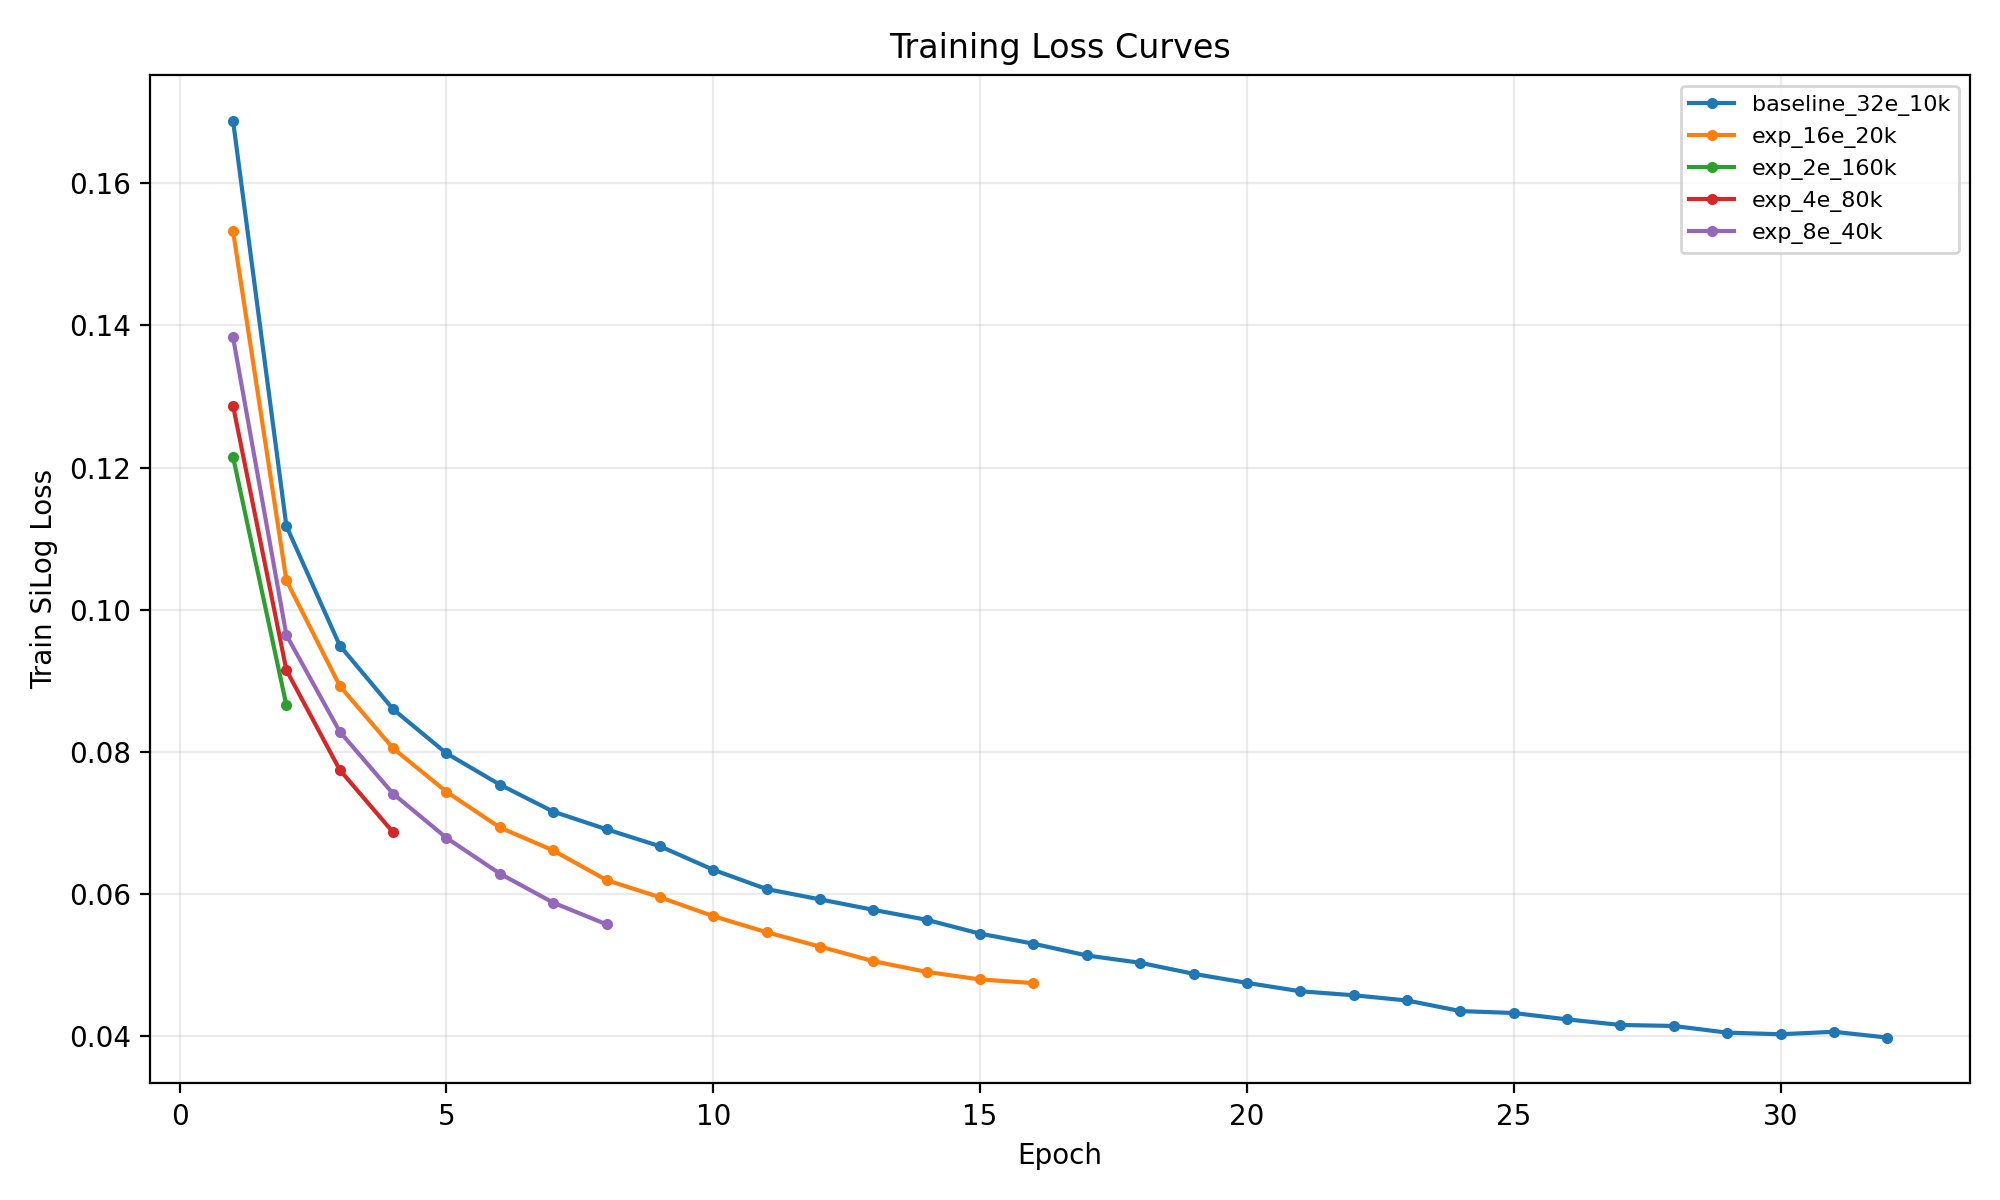
\includegraphics[width=\linewidth]{../task3/outputs/pic/train_loss_curves.png}
      \caption*{(a) Training loss curves}
   \end{minipage}
   \hfill
   \begin{minipage}{0.49\linewidth}
      \centering
      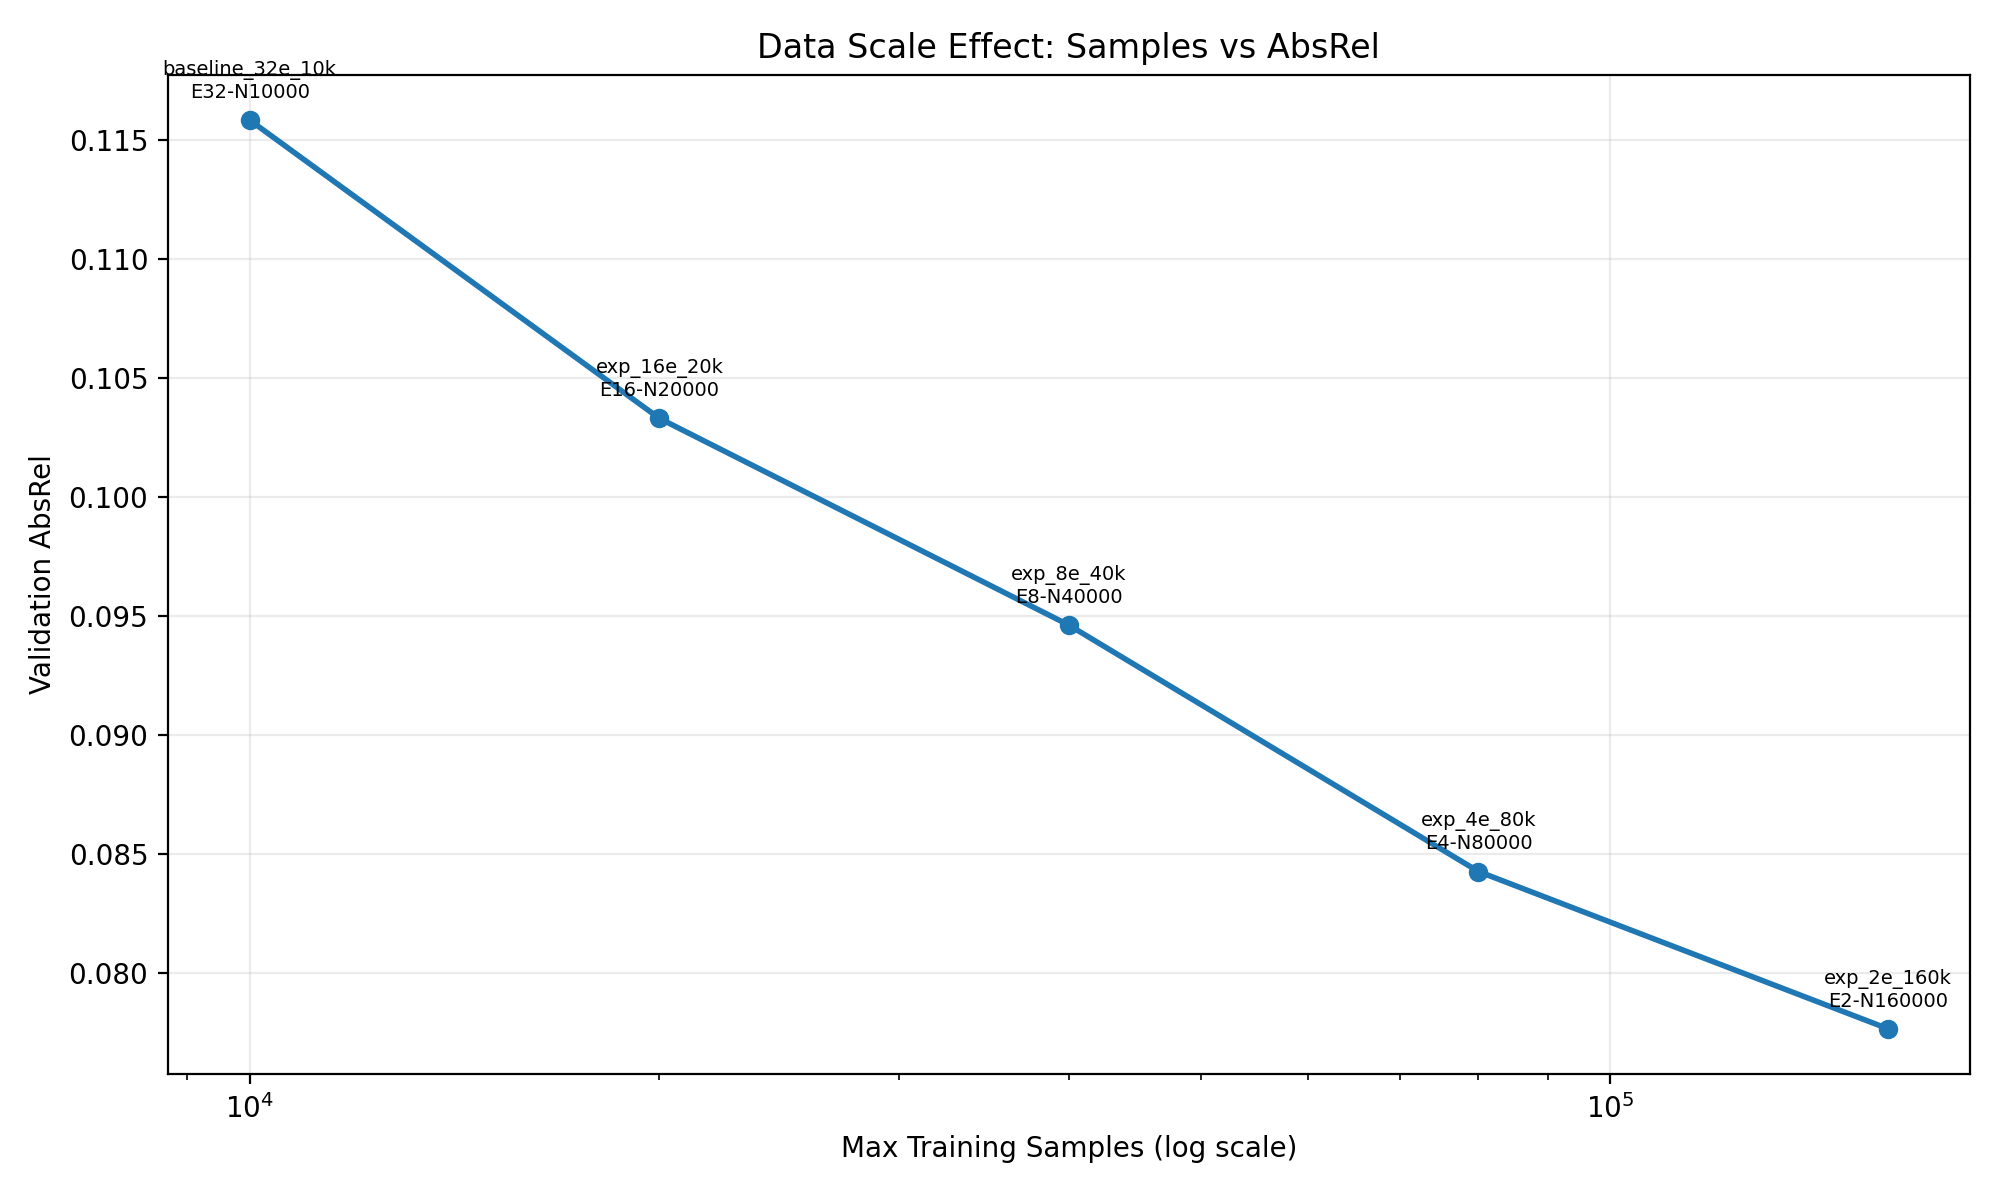
\includegraphics[width=\linewidth]{../task3/outputs/pic/data_scale_effect.png}
      \caption*{(b) Data scale effect}
   \end{minipage}
   \caption{Task 3 training dynamics and effect of sample scale.}
   \label{fig:task3_train}
\end{figure}

As shown in Fig.~\ref{fig:task3_train}(b), increasing sample count under shorter epochs continuously improved validation AbsRel in this experiment (from 0.1158 to 0.0777), indicating that broader data coverage can be more beneficial than longer optimization on a smaller subset.

\paragraph{Foundation Model Comparison}
I evaluated two foundation models, VGGT~\cite{vggt_arxiv} and Depth Anything 3 (DA3)~\cite{da3_arxiv}, using the same evaluation protocol in \texttt{test.py}.

\begin{figure}[htbp]
   \centering
   \begin{minipage}{0.49\linewidth}
      \centering
      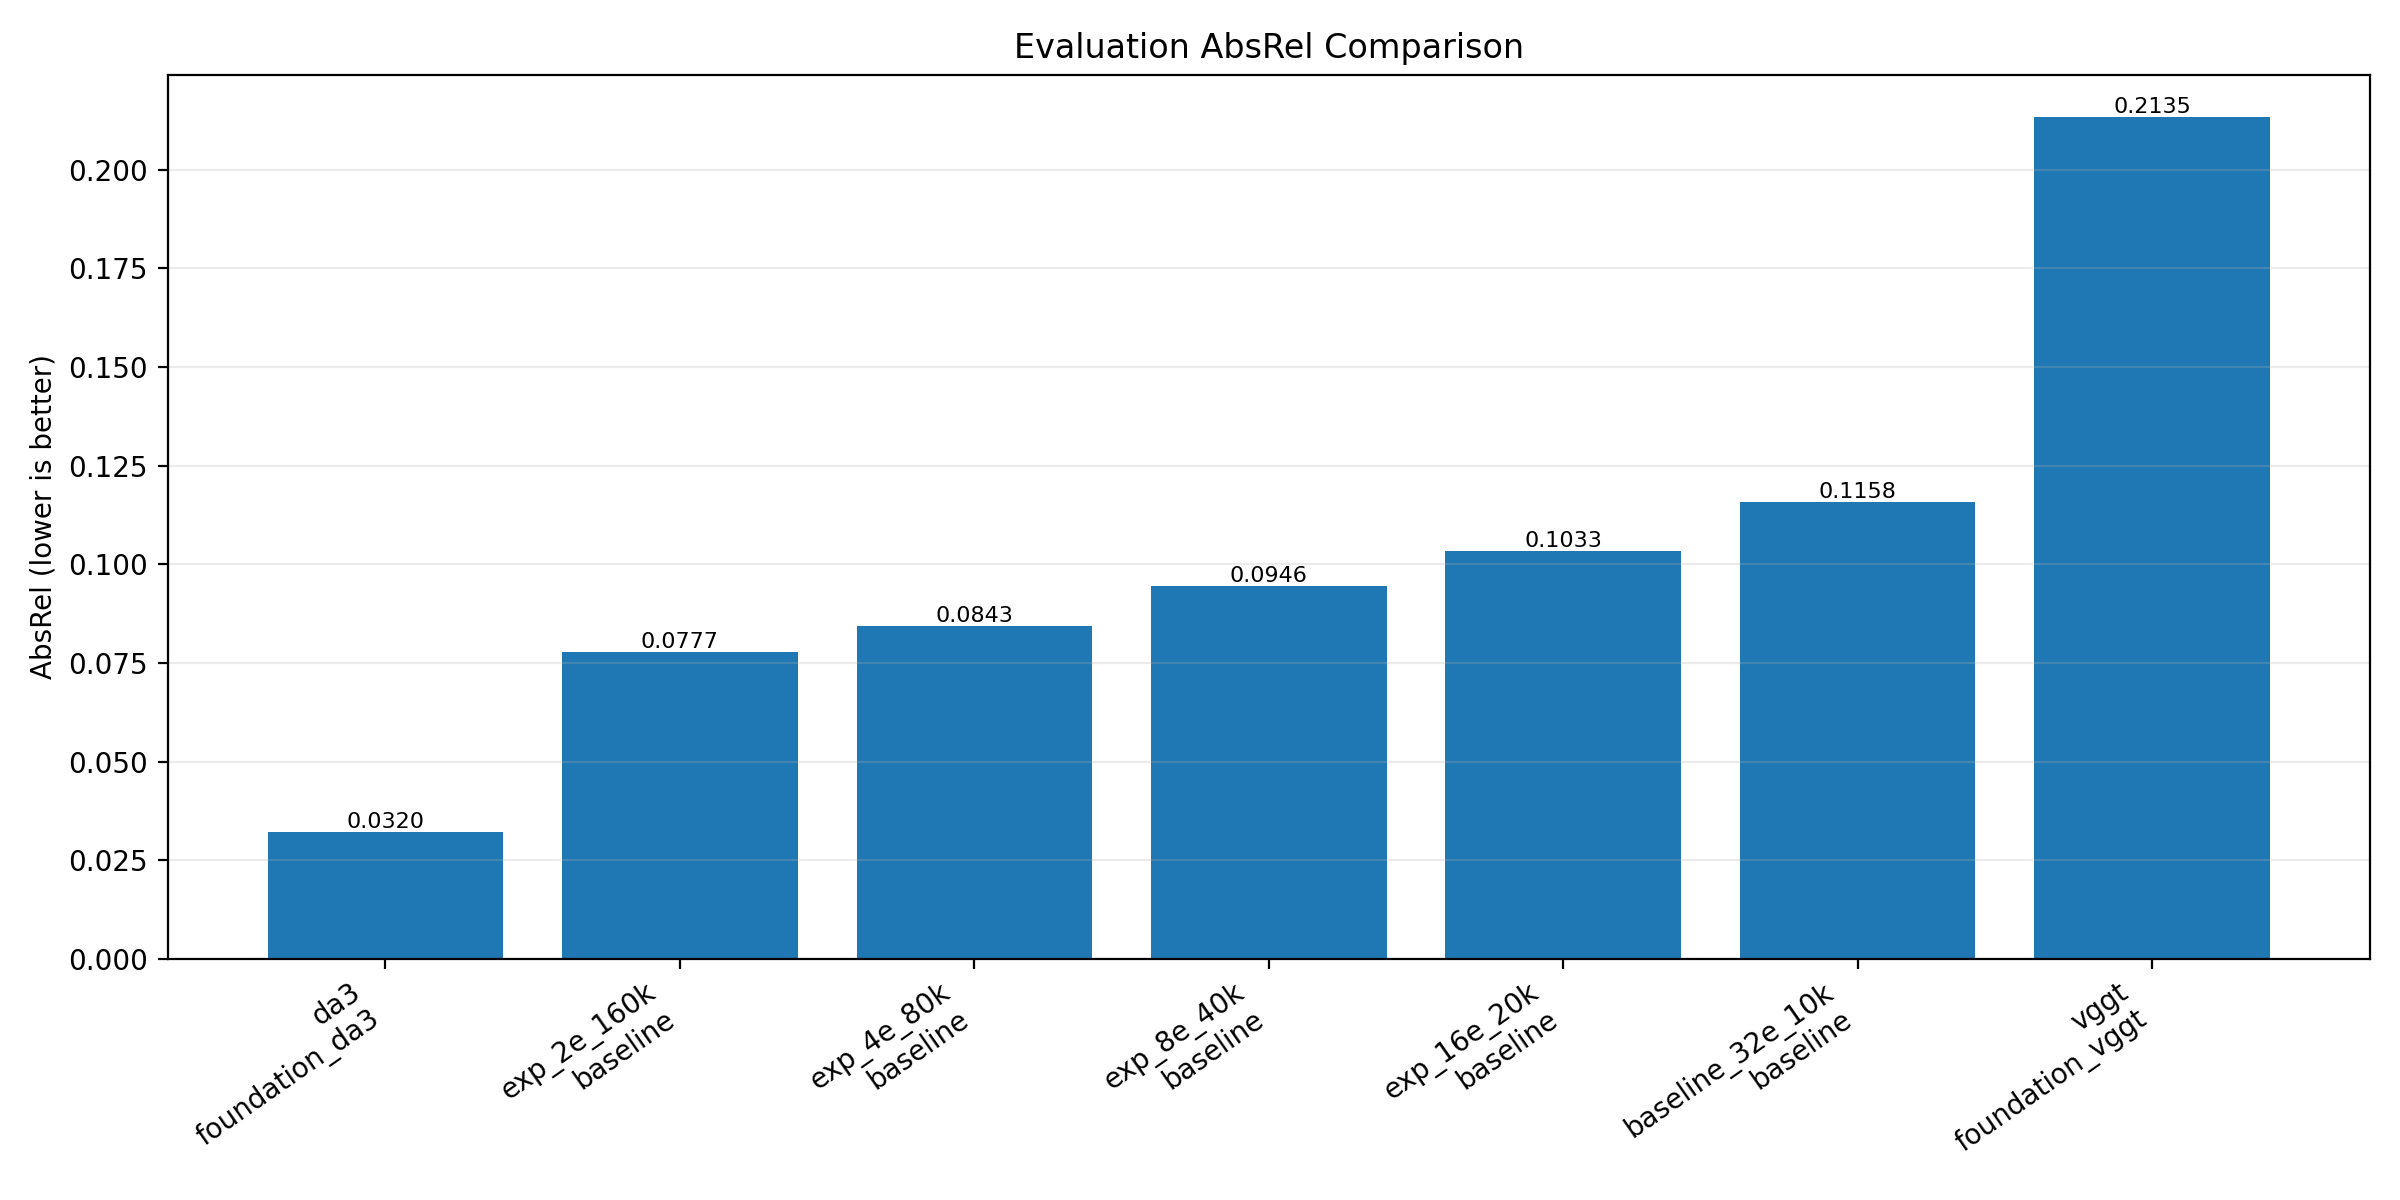
\includegraphics[width=\linewidth]{../task3/outputs/pic/eval_absrel_bar.png}
      \caption*{(a) Overall AbsRel comparison}
   \end{minipage}
   \hfill
   \begin{minipage}{0.49\linewidth}
      \centering
      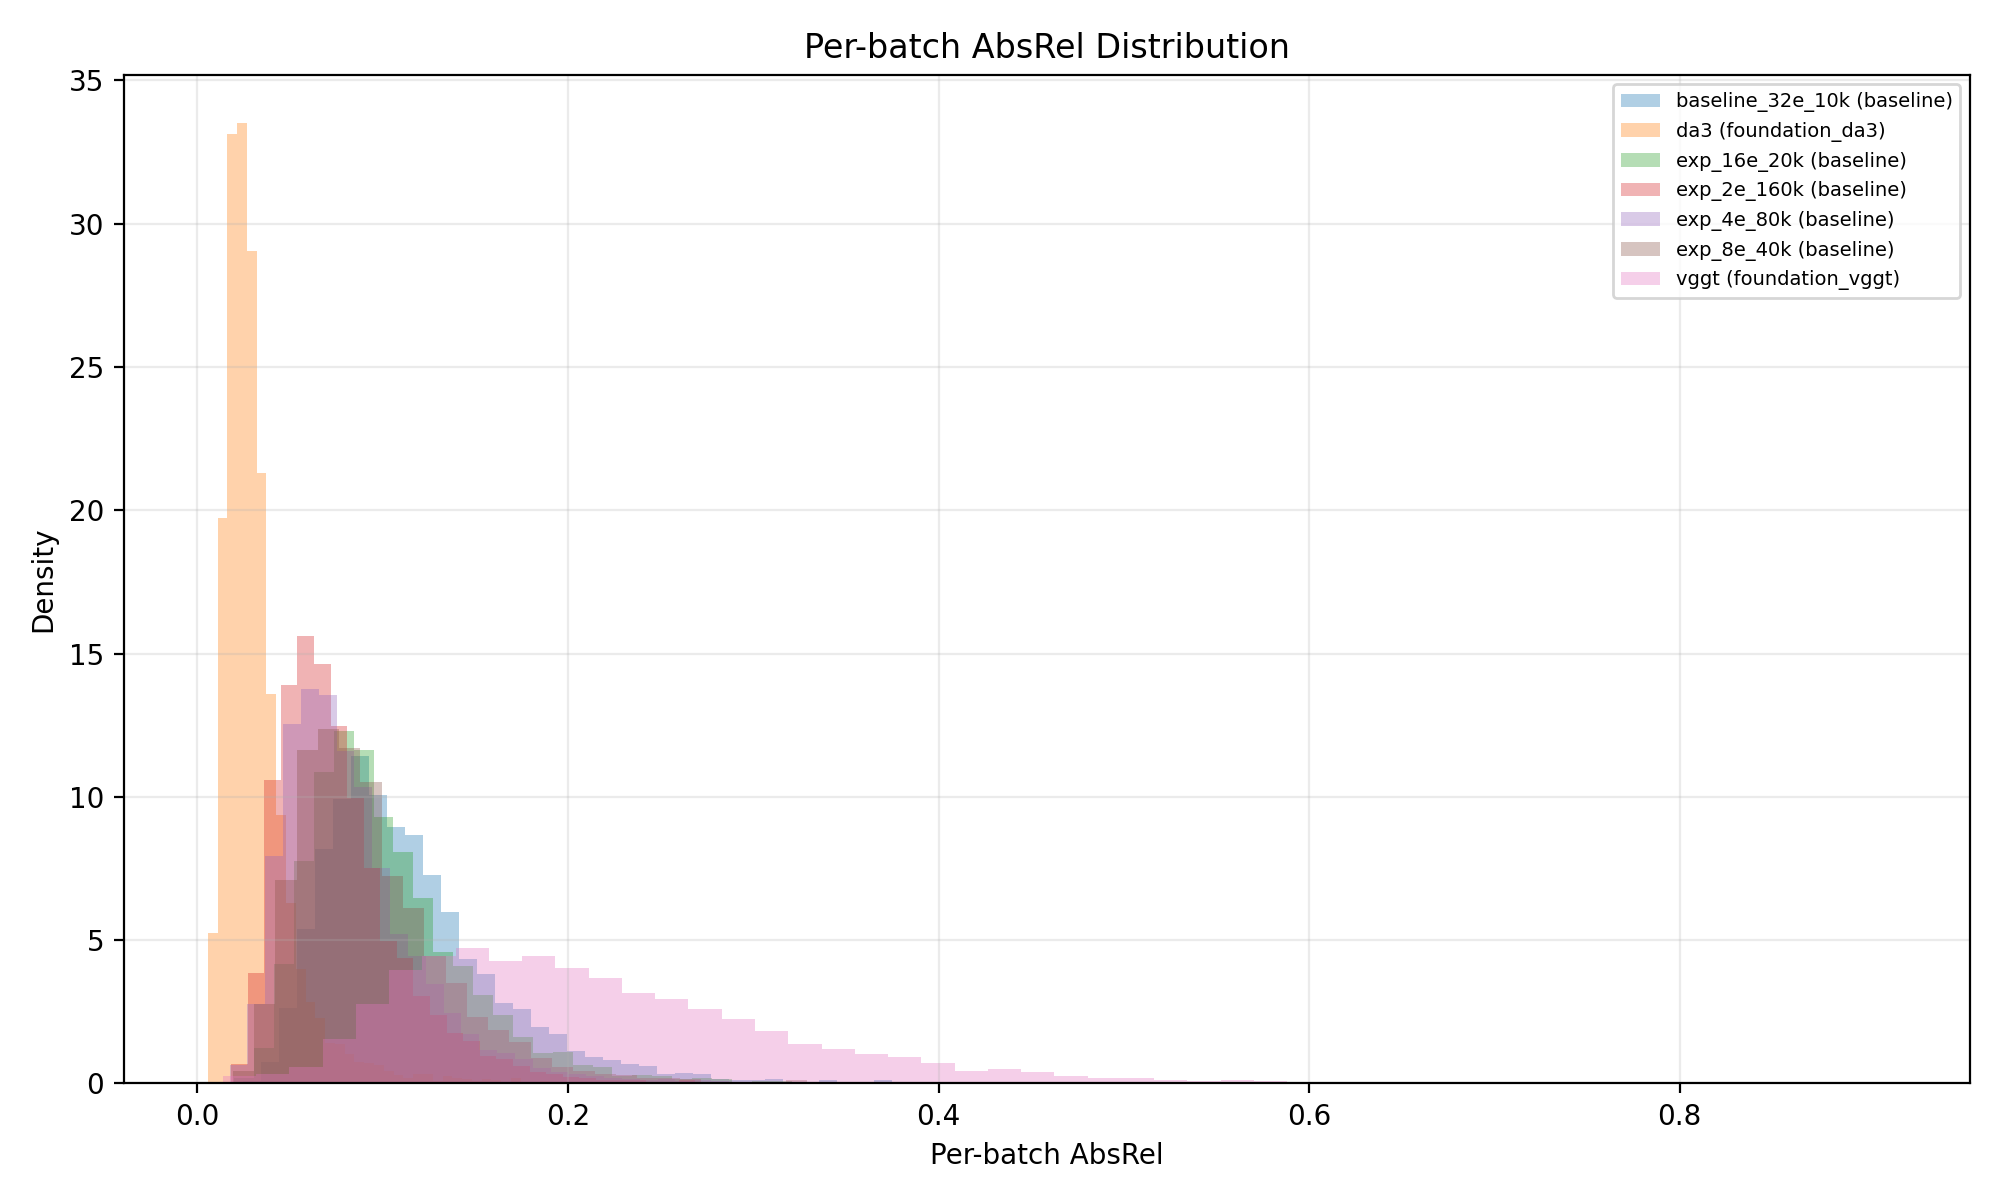
\includegraphics[width=\linewidth]{../task3/outputs/pic/eval_per_batch_hist.png}
      \caption*{(b) Per-batch distribution}
   \end{minipage}
   \caption{Task 3 quantitative comparison across baseline/data-scale/foundation methods.}
   \label{fig:task3_eval}
\end{figure}

\begin{table}[htbp]
\centering
\small
\begin{tabular}{lcc}
\toprule
Method & Setting & AbsRel (val) \\
\midrule
Baseline & 32e, 10k samples & 0.1158 \\
Baseline & 16e, 20k samples & 0.1033 \\
Baseline & 8e, 40k samples & 0.0946 \\
Baseline & 4e, 80k samples & 0.0843 \\
Baseline & 2e, 160k samples & 0.0777 \\
VGGT & foundation\_vggt & 0.2135 \\
DA3 & foundation\_da3 & 0.0320 \\
\bottomrule
\end{tabular}
\caption{Task 3 quantitative results (aligned AbsRel, lower is better).}
\label{tab:task3_results}
\end{table}

In this setup, DA3 achieved the best AbsRel, while VGGT underperformed the baseline. A likely reason is that different foundation models have different preferred input formats and operating assumptions, and performance is sensitive to adaptation details in downstream evaluation scripts.

\section{Conclusion}

This assignment covers three levels of vision tasks: low-level filtering, contrast enhancement, and high-level depth estimation. Task 1 and Task 2 confirm that implementing classical methods from first principles helps understand how parameters and local statistics affect visual quality. In Task 3, the controlled experiments show clear data-scale trends for baseline training and highlight the impact of model adaptation when comparing with foundation models. The full pipeline (training logs, evaluation JSON, and plotting scripts) is reproducible and can be extended for further benchmarking.

{\small
\bibliographystyle{ieee_fullname}
\bibliography{egbib}
}

\end{document}
